\section{Preliminaries}

\subsection{Concepts}
\begin{figure}[t!]
\centering
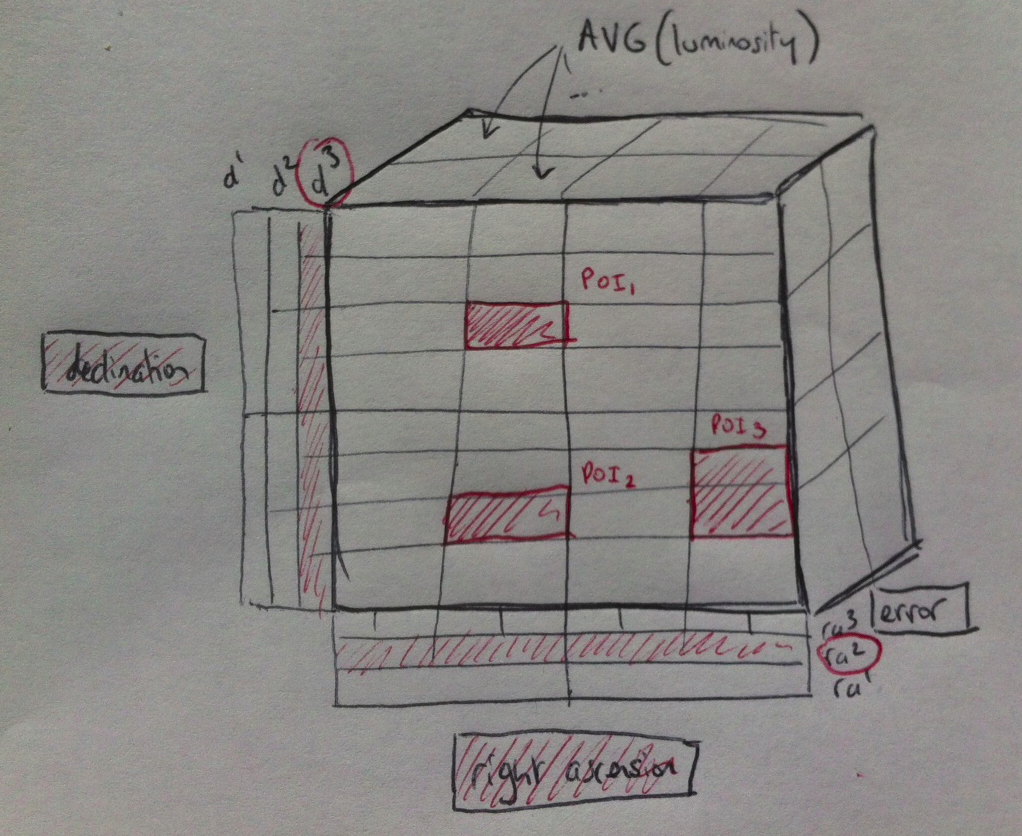
\includegraphics[width=0.9\columnwidth]{images/cube}
\caption{Example of recommendation}
\label{cube}
\end{figure}
We model the database as a large relation $DB$. This table contains two types
of columns: the dimensions $D_0, \ldots, D_d$ and a target column $T$. The
target column contains the target value for each tuple. Note that this view is
logical: we are oblivious to the physical structure of the data.  Claude's aim
is to generate a set of \textbf{explanations}.  An explanation contains two
elements: a \textbf{view} and several \textbf{points of interest} (POI). A view
is an ``informative'' set of dimensions, on which we project the data.  A point of
interest is a selection over this view. It contains tuples for which the target
has a ``remarkable'' distribution.

We illustrate these concepts with Figure \ref{cube}. Our example database
describes light sources.  It contains three dimensions: \texttt{right
ascension}, \texttt{declination} and \texttt{error}. The first two describe a
source's position. The third one describes the measurement errors. For each
tuple, we target the value of the column \texttt{brightness}. Claude's output
is highlighted in red. It contains a view based on \texttt{right ascension},
and \texttt{declination}. We see that the view is a SQL query with the
following structure:
\begin{verbatim}
SELECT   D1, ... , Dn , AVG(T)
FROM     DB 
GROUPBY  D1, ... , Dn
\end{verbatim}
The $n$ distinct variables $\texttt{D1} \ldots \texttt{Dn}$ define the view. Once
Claude has chosen a view, it must explain \emph{why} it has chosen this view.
This is the role of POIs. In Figure \ref{cube}, Claude suggests three POIs. We
can express them in SQL as follows:
\begin{verbatim}
SELECT   AVG(T)
FROM     DB
WHERE    D1 BETWEEN l1 AND h1
 AND     ...
 AND     Dn BETWEEN ln AND ln
\end{verbatim}
The POIs are defined by the ranges $\texttt{[l1,h1]}, \dots \texttt{[ln,hn]}$.


\subsection{Informative explanations}
\label{sec:infor}
\begin{figure}[t!]
\centering
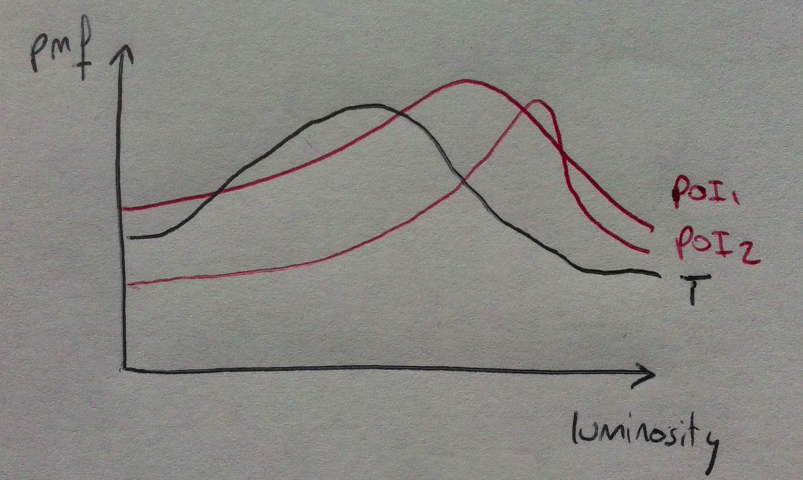
\includegraphics[width=\columnwidth]{images/poi}
\caption{The POIs have unusual distributions}
\label{poi}
\end{figure}

We defined Claude's search space: we want to suggest views and POIs. We now
present how the target helps us recognize the ``interesting'' ones. 

First let's explain how to choose the views. A set of columns is informative if
it is somehow related to the target: if we filter the data on these columns,
the target value changes.  We model this relationship with statistical
dependency. We represent each  dimension $D_k$ by a random variable $\rv{D}_k$.
We model the target with a random variable $\rv{T}$.  A view is interesting if
there exists some statistical dependency between its columns and the target. We
formalize this statement with Mutual Information \cite{cover2012elements}:

\begin{definition}
Consider a view $V = \{D_1, \ldots, D_n\}$, and the target column $T$.  Let
$I$ denote the \emph{Mutual Information} between two random variables. We
define the \textbf{strength} of $V$ as follows:
\[\sigma(V) = I(\rv{D}_1, \ldots, \rv{D}_n ; \rv{T})\]
\end{definition}

{\color{red}
Detail what the MI is, how to compute, etc...
}

Claude seeks variables which are \emph{jointly depdendent} to the target. We
measure dependency with the mutual information, because this quantity is
general (correlation is only one type of dependency).

The next step is to extract the POIs. The POIs contain tuples for which the
measure have an ``unusual'' distribution compared to the rest of the database.
Consider Figure \ref{poi}. The curves show the probability mass function of the
brightness for three sets of tuples: the whole database, $POI_1$ and $POI_2$.
The sets $POI_1$ and $POI_2$ come from the view \texttt{right ascension -
declination} in Figure \ref{cube}. We observe that they deviate from $DB$.
They illustrate how right ascension and declination can influence brightness.
We quantify this observation with the Kullback-Leibler divergence:

\begin{definition}
Consider a range $R = [l_1, h_1] \times \ldots \times [l_n, h_n]$. 
The random variable $\rv{T}_R$ describes the target for
the tuples in $R$, and $\Pr(\rv{T}_R)$ its distribution.
We define the \textbf{divergence} of the range $R$ as follows: 
\[\delta(R) = KL \big( \Pr(\rv{T}) \| \Pr(\rv{T_R})  \big)\]
\end{definition}

The Kullback-Leibler divergence measures the difference between two probability
distributions. Our function $\delta$ grows when a range has unsual target
values, it decreases otherwise. It does not target specifically high or low
values. It seeks \emph{any} type of deviation from the target's global
distribution.  Note that divergence is tightly related to strength:

\begin{lemma}
Let $V$ denote a view. We create a grid over $V$ by discretizing its
columns. The variable $\rv{R}$ describes a random cell.  We observe the
following relationship:
\[
    \sigma(V) = \mathbb{E}_{\rv{R}} \{ \delta(\rv{R}) \}
\]
\end{lemma}

\begin{proof}
Let $\rv{V}$ represent the joint distribution $\rv{D}_1, \ldots, \rv{D}_n$.
We have $\sigma(V) = I(\rv{V},\rv{T})$.
By definition of the Kullback-Leibler divergence, we have: 
$I(\rv{V},\rv{T}) = $ $\mathbb{E}_{\rv{V}} \{ KL( \Pr(\rv{T} | \rv{V}) \|$ $ \Pr(\rv{T}) ) \}$
As the data is discretized, $\rv{V}$ and $\rv{R}$ are equivalent. Also,
for any bin $R$, $\Pr(\rv{T} | \rv{V} = R)$ is equivalent to
$\Pr(\rv{T}_R)$. We derive the lemma.
\end{proof}


This lemma is simple but powerful. It shows that strength and divergence are
``two sides of the same coin'': the strength of a view equals exactly the
average divergence of its bins. We use the terms strength and
deviation interchangeably to characterize an \emph{explanation} (recall that a
explanation contains both the view and its POIs).

\begin{definition}
Let $S=(\{ D_1, \ldots, D_n\}, \{R_1, \ldots, R_r\})$ describe an explanation . The
\textbf{strength} (or \textbf{divergence}) of $S$ equals the strength
of its view.
\end{definition}

We are now ready to formulate our problem.

\begin{problem}
Consider a dataset $DB$, a target column $T$ and a triplet $(q, n, r)$. Find
the top $q$ strongest explanations, with $n$ variables and $r$ POIs.
\end{problem}

To solve this problem, Claude operates in two steps. First, it detects $q$
strong sets of columns.  We call this step \emph{column search}.  Then comes
the \emph{POI dectection} step: for each view we extract $r$ POIs. In practice,
our top $q$ strategy can generate redundancy. We tackle this problem with an
optional \emph{refinment} step.

\section{Column selection}
\label{sec:colum}

{\color{red} 
This section requires some reordering.
\begin{itemize}
    \item Introduce Lemma 2, and the idea to search for columns greedily
    \item Present the exact approach
    \item Present the approximation
\end{itemize}
Also, the description of the approximation should be deepened.
}

The aim of this phase is identify the $q$ strongest sets of variables. From
here on, we use the notations $D_i$ and $\rv{D}_i$ interchangeably - we can use
the context to distinguish database columns and random variables.

\subsection{Base algorithm}
\begin{figure}[t!]
\centering
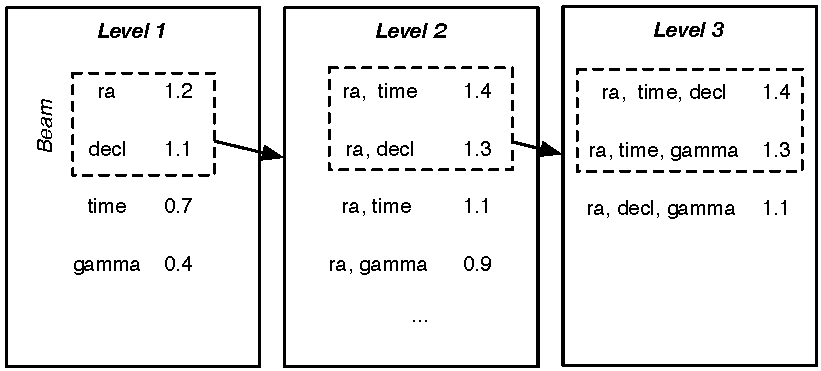
\includegraphics[width=0.8\columnwidth]{images/beam-search}
\caption{Example of Beam Search, with a beam size of 2}
\label{pic:beam-search}
\end{figure}

To recommend views, Claude must find the best sets of at most $n$ variables.
The search space of this problen grows exponentially with $n$: from a database
with $d$ variable, we can generate $\sum_{i \leq n} \binom{d}{i}$ combinations.
Besides, there is to our knowledge no bound which would allow us to prune the
search space efficiently. 

We propose to use level-wise search. To initialise the algorithm, we compute
the strength of each variable separately (we compute $\sigma(D_i) = I(D_i;
T)$). We order the candidates, and keep the top $b$ variables. We call this set
the \emph{beam}. We then form new candidates by appending each variable of the
database to each variable in the beam. We obtain views with two columns. We
compute the best $b$ results and update the beam. The procedure is repeated
until the beam contains views with $n$ variables. We illustrate the procedure
in Figure \ref{pic:beam-search}.

\begin{figure}[t!]
\centering
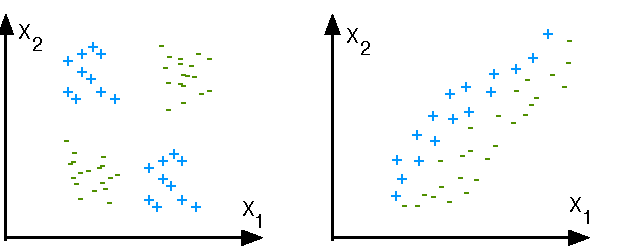
\includegraphics[width=0.8\columnwidth]{images/strength-jump}
\caption{Limit cases of the beam search strategy. The variables $var1$ and
$var2$ represent two dimensions. The symbol and color of the plots represent
the value of the target class. }
\label{pic:strength-jump}
\end{figure}
Thanks to our beam strategy, we avoid exploring an exponentially large search
space. Instead, we compute the strengths of at at most $n.b$ settings.
Unfortunately, this strategy induces an accuracy penalty: if the beam is too
small, we may miss some good candidates. This is a consequence of the following
observation: a set of columns which is outside the top $q$ candidates at step
$i$, could very well appear in the top $q$ at step $i+1$. Consider for instance
the two classic scenarios pictured in Figure \ref{pic:strength-jump}. The
dimensions $var1$ and $var2$ taken in isolation are weak: we can infer no
useful information about the target from either of them. However, their
combination is very interesting.  This observation is reflected by the
strength: the views $\{var1\}$ and $\{var2\}$ have a very poor strength, but
$\{var1, var2\}$ is an excellent candidate. If use a beam search strategy, we
may discard  $\{var1\}$ and $\{var2\}$ early because they have a low score.
This would be a mistake, because we lose the opportunity to discover $\{var1,
var2\}$.

\subsection{Approximating the View Strength}
\label{sec:approx}


The Beam Search aslgorithm gives us a convenient way to find good views.
Through the size of the beam, we can find a compromise between execution time
and accuracy.  Nevertheless, the algorithm is still too heavy for an
interactive application. For each candidate, it computes the mutual information
between all the variables of the view and the target, which involves heavy grouping
operations. Our solution is to \emph{approximate} the strength of the views
during the iterations of the algorithm. Then, we use exact calculations for the
final ranking.

To present our approximation scheme, we must first describe how a
view is impacted when we add a column to it.

\begin{lemma}\label{lem:chain}
Consider a view $V = \{D_1, \ldots, D_i\}$, and a target $T$.
For any column $D_{i+1}$: 
$$
\sigma(V \cup \{D_{i+1}\}) =  \sigma(V) + I(D_{i+1} ; T | D_1 , \ldots, D_i)
 $$
\end{lemma}
\begin{proof}
This lemma is a direct consequence of the Mutual Information's chain rule
\cite{cover2012elements}.
\end{proof}

This lemma describes how much a view improves if we append a new dimension.
For any random variables $X,Y,Z$, the notation $I(X;Y|Z)$ expresses the
\emph{conditional mutual information}. It describes the dependency between $X$
and $Y$, \emph{given $Z$}. The influence of $Z$ can go either way: it can
weaken or strengthen the relationship between $X$ and $Y$. In any case, it is
positive or null, and it is bounded by the entropy of $X$ and $Y$.

In practive, computing $ I(D_{i+1} ; T | D_1 , \ldots, D_i)$ is not less
expensive than calculating the strength of $\{D_1, \ldots, D_{i+1}\}$ directly.
But we can use the following approximation:
\[
\begin{split}
    \sigma(V \cup \{D_{n+1}\}) & = \sigma(V)   + I(D_{n+1} ; T | D_0, \ldots, D_{n})\\
                           & \approx \sigma(V) + I(D_{n+1} ; T | D_{i})
\text{ for } D_i \in V
\end{split}
\]

The idea behind this approximation is naive: we assume that $I(D_{n+1} ; T |
D_0, \ldots, D_{n}) \approx I(D_{n+1} ; T | D_{i})$. We ignore the high order
dependencies. Thanks to this assumption, we can compute the strength of a view
much faster.  Consider a directed graph in which each vertex represents a
variables $D_i$. Each edge $(D_i, D_{i+1})$ has a a weight $ I(D_{i+1} ; T |
D_{i})$.  We call this graph \emph{co-dependency} graph.  To compute the
approximate strength of ${D_0, \ldots, D_i}$, we build a spanning tree which
covers all the vertices of the view, and sum the weights of the edges.

In most cases, we can build several different spanning trees with different
weights. Which one should we use? We could use two variants. An
\emph{optimisic} approximation $\sigma_+ $ would consider the \emph{maximum}
spanning tree.  A \emph{pessimistic} approximation $\sigma_- $ would use the
weight of the \emph{minimum} spanning tree. For the rest of this paper, we will
only consider the latter aleternative. 

We now present a faster version of our view search algorithm.  We operate in
two steps. First, we compute the strength of every column and every couple of
columns.  This gives us a first set of candidates, and we can derive the
co-dependency graph using the fact that $I(D_{j} ; T | D_i) = \sigma(D_i ;
D_{j}) - \sigma(D_i)$.  Then, we run Beam Search as previously, but with the
approximate strength computation.  To append the variable $D_i$ to the view
$V$, we list every edge which connects  $D_i$ to the columns of $V$. We
identify the lightest one and add the value of its weight to $\sigma(V)$.  

This algorithm is much faster because it spares us expensive database
operations. Instead, we perform computations on a graph with $d$ nodes.  To
save some accuracy, we use the exact version of the view strength for the final
top $q$ ranking.

\section{Detecting Points Of Interest}
\label{sec:detec}

During this phase, we find the $r$ most divergent regions for each view.
Fortunatly, this task is an instance of a known Data Mining problem,
\emph{Subgroup Discovery} \cite{klosgen1996explora}\cite{wrobel1997algorithm}.
The aim of Subgroup Discovery is to identify sets for which the target value
maximizes a user-defined quality measure. To solve our problem, we instantiate
the quality measure with the divergence.

In principle, we could use any efficient algorithm from the Subgroup Discovery
litterature.  We propose to reuse the beam Search strategy from the previous
section, but to explore \emph{tuples} instead of columns. We bin the data in a
coarse manner and get a first set of $b$ cells. We then refine these cells with
a thinner binning, etc...

As mentioned in the Subgroup Discovery litterature \cite{van2011non}, our
divergence score has a drawback: it favours smaller groups.  Therefore, Beam
Search may converge very late or not at all.  A practical
solution is to alter the model to take the size into account. Let $R$
represents a range with cover $|R|$, and $|V|$ represent the number of tuples
in the view. We use the \emph{weighted} deviation $\delta_w(R) = |R|/|V| \times
\delta(R)$. This new score introduces a penalty for small POIs.


\section{Improving the Diversity of the Views}

{ \color{red} This section should go. Instead, replace it with a few mentions
to deduplication in the previous section and/or in the experiments}

As Claude is based on a top-k approach, its output may be redundant: the views
may be very similar to each other.  Some users prefer small but diverse sets of
suggestions.  We tackle this problem with compression techniques from the
frequent petterns literature. For instance, the Krimp algorithm is an
established strategy, based on the Minimum Description Length principle
\cite{vreeken2011krimp}. Another approach would be to cluster the views, and
return one representative view per cluster.


\section{Use Cases}

\subsection{Criminality}

\begin{figure*}[t!]
    \centering
    
    \begin{subfigure}[b]{\textwidth}
    \includegraphics[width=\textwidth]{plots/ViolentCrimesExample1}
    \caption{Fully worked out example 1}
    \label{fig:violent-example1}
    \end{subfigure}

    \begin{subfigure}[b]{\textwidth}
    \includegraphics[width=\textwidth]{plots/ViolentCrimesExample2}
    \caption{Fully worked out example 2}
    \label{fig:violent-example2}
    \end{subfigure}

\label{pic:violent-example}
\end{figure*}

\begin{table}[position specifier]
  \centering
\begin{tabular}{l c}
    \hline
    View & Score (bits) \\
    \hline
    Police.Overtime, Pct.Vacant.Boarded, & 0.88\\
    Pct.Race.White & \\
    Pct.Families.2.Parents, Pct.Race.White, & 0.84\\
    Police.Requests.Per.Officer & \\
    Pct.Police.White, Pct.Police.Minority, & 0.64\\
    Pct.Vacant.Boarded &\\
    Pct.Empl.Profes.Services, Pct.Empl.Manual & 0.64\\
    Pct.Police.On.Patrol & \\      
    Pct.Retired, Pct.Use.Public.Transports & 0.61 \\
     Pct.Police.On.Patrol & \\ 
    Pct.Recently.Moved, Population.Density & 0.60 \\
    Police.Cars & \\
    \hline
\end{tabular}
\caption{Examples of views from the Crime example.}
  \label{tab:crime_views}
\end{table}

\section{Experiments}

{\color{red}
The graphs should be simplified. Instead, use tables.
}

We use real data sets from the UCI repository and KIT, with different
charatetistics. We interrupt experiments which last more than 30 minutes.
Claude is implemented in R, but the information theory primitives are written
in C.

In the following sections, we will use the \emph{normalized} version of view
strength: instead of displaying $\sigma(V)$, we show $\sigma(V) / H(T)$ (recall
that $\sigma(V) \in [0, H(T) ]$).

\subsection{View strength and prediction}

\begin{figure}[t!]
\centering
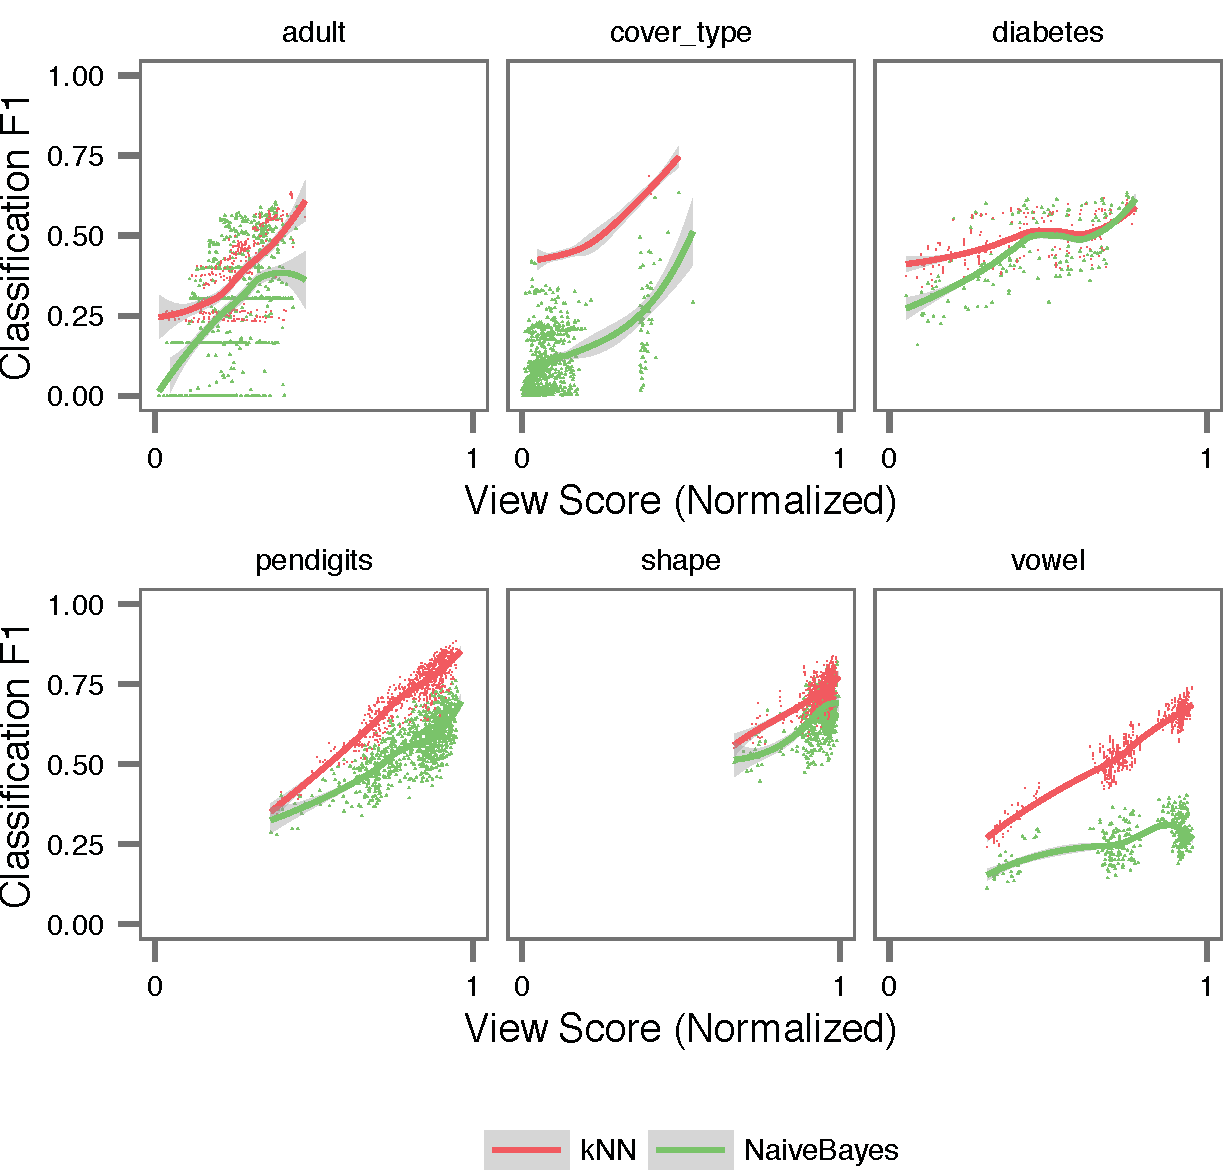
\includegraphics[width=\columnwidth]{plots/compare-strength-f1}
\caption{Strength vs. Classification accuracy for 1,000 random views. The blue
    and red lines represent local regressions, computed on a sliding window of
    80 points. The grey shade around the lines represents a 90\% confidence
interval.}
\label{pic:strength-vs-f1}
\end{figure}

In this set of experiments, we examine how interesting strong views really are.
To do so, we simulate the users with statistical classifiers.  We generate
1,000 random views for each dataset. We compute the strength of the views, and
measure how well the classifiers perform with them. If the classifiers have a
low performance with weak views and a high performance with strong views, then
our approach is validated. We use two different classifiers: 3-NN, and Naive
Bayes.  These approaches are known to be simple, efficient, and they have no
built-in mechanism to filter irrelevant variables (as opposed to decision
trees). To measure their performance, we use 10-fold cross-validation.

For all our datasets we observe that the classifier's F1 grows with the
strength of the views. We present the results for six datasets in Figure
\ref{pic:strength-vs-f1}. Clearly, the view strength has a positive influence
on accuracy. This confirms our approach: a strong view contains all the
information necessary to understand how the target varies. 


\subsection{View Selection}

{\color{red}
    We need more baselines here.
    \begin{itemize}
        \item The wrapper based on Naive Bayes
        \item A feature selection algorithm
        \item HiCS?
     \end{itemize}
}


\begin{figure*}[t!]
\centering
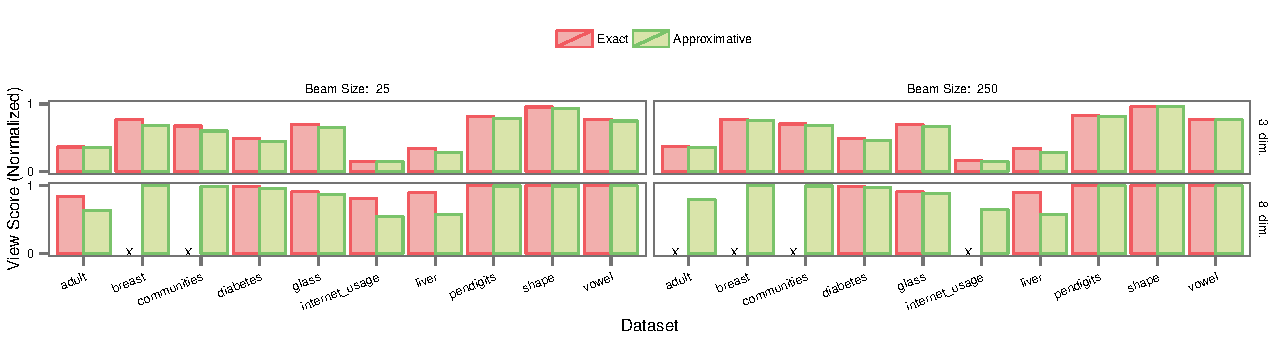
\includegraphics[width=2\columnwidth]{plots/column-select-score}
\caption{Performance of the View Selection Algorithms with different view and
beam sizes. The symbol \texttt{x} represents a missing value.}
\label{pic:column-select-score}
\end{figure*}
 
\begin{figure*}[t!]
\centering
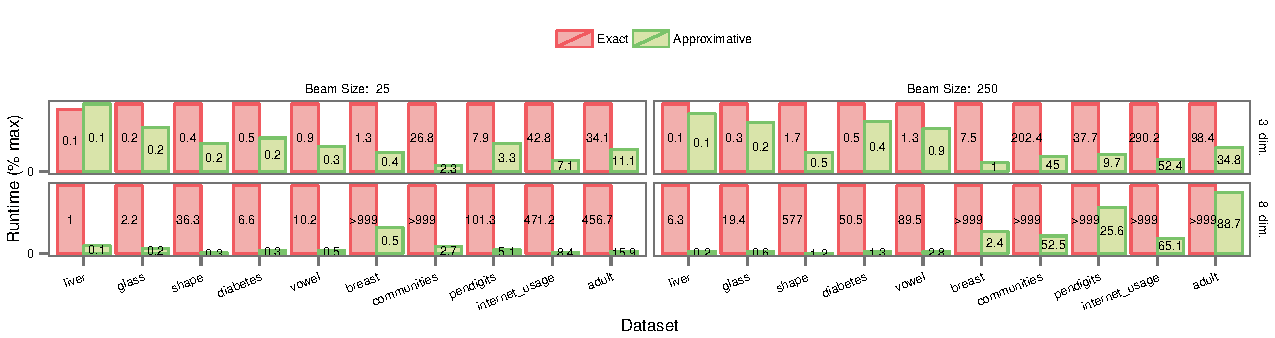
\includegraphics[width=2\columnwidth]{plots/column-select-time}
\caption{Runtime of the View Selection Algorithms. The symbol \texttt{x}
indicates that the experiment breached our 15 minutes threshold.} 
\label{pic:column-select-time}
\end{figure*}

We now evaluate our view selection strategy. We compare two approaches, both
based on beam search. The first approach uses the exact strength computations.
The second approach use the approximation described in \ref{sec:approx}. Figure
\ref{pic:column-select-score} shows the average score of the top 25 views
returned by both approaches. In almost all cases, the approximation does induce
a very slight penalty. Also, we note that the size of the beam has little to no
influence on the results. This hints that Beam Search is an efficient
heuristic: we do not need to explore the whole search space to find good
solutions.

Figure \ref{pic:column-select-time} describes the runtime of each strategy. It
shows that our solultion is extremely efficient: the view search based on
approximations is up to two orders magnitude faster than its competitor. To
explain this, recall that the ``exact'' algorithm must scan the
whole database to evaluate the strength of each view. The approximate algorithm
only performs a few lookups on the co-dependency graph.

\subsection{View and POIs}

\begin{figure*}[t!]
\centering
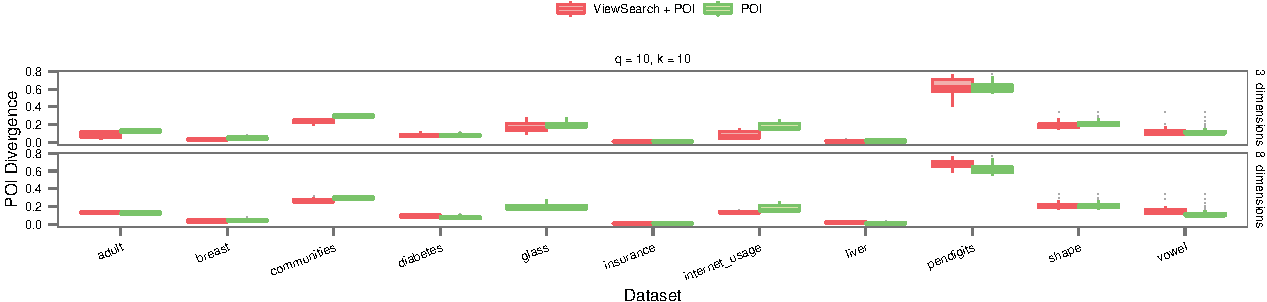
\includegraphics[width=2\columnwidth]{plots/View-POI-Acc}
\caption{Quality of the POIs returned by Claude, for different q, k and n.}
\label{pic:quali-POIs}
\end{figure*}
 
\begin{figure*}[t!]
\centering
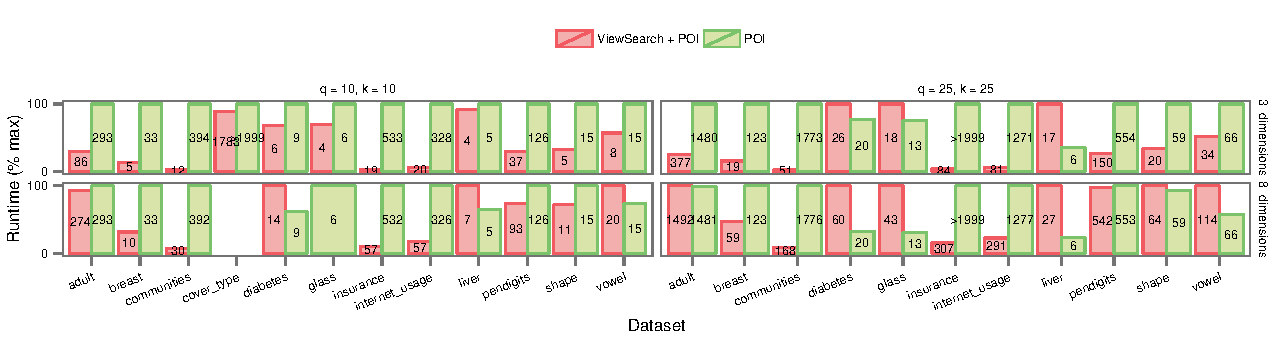
\includegraphics[width=2\columnwidth]{plots/View-POI-Time}
\caption{Execution time of Claude versus Beam Search for different q, k and n.} 
\label{pic:time-POIs}
\end{figure*}

Figures \ref{pic:quali-POIs} and \ref{pic:time-POIs} present our evaluation of
Claude's POIs. We compare two approaches. The algorithm \texttt{View Search +
POI} is Claude's natural approach, presented in the paper. First we search $q$
views, then we return $k$ POIs per view. The idea behind \texttt{POI} is to
apply Beam Search on the whole database directly. Instead of seeking $k$ POIs
in $q$ projections, we seek $q.k$ selections from the full column space.  We
skip the view selection step. Ths strategy is used by many state-of-art
subgroup discovery algorithms. 

Figure \ref{pic:quali-POIs} describes the quality of the POIs. In most case, we
observe that difference is very subtle. The \texttt{POI} approach tends to give
better results for low $q$ and $k$ and small views (llustrated by the top left
corner of the Figure). When $q$, $k$ and $n$ and higher, Claude tends to find
better POIs.

Claude's advantage comes from its runtime. In Figure \ref{pic:time-POIs}, we
see that in many cases, Claude is at least twice as fast as the pure Beam
Search approach. As Claude decouples view search and POI search, it
overperforms state of the art Subgroup Discovert techniques.

Last minute comment: it seems that the price to pay is redundancy. It is
possible to obtain the \emph{same subgroup} from \emph{different views}. The
description is different, but the tuples are the same. Thereore Claude's POIs
are even more redundant that those obtained by normal Subgroup Discovery.  This
could explain why the KL deviations are overall so high.
